\begin{frame}
    \frametitle{Strip-packing problem}
    \framesubtitle{}
    \begin{figure}[H]
        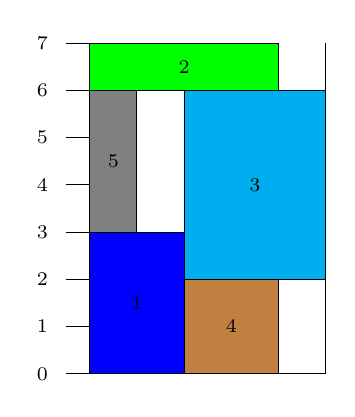
\begin{tikzpicture}[scale=0.6]
        \tikzstyle{every node} = [font=\scriptsize]
            \begin{scope}
                \foreach\x in {0,1,...,7}{
                    \draw (-0.5,\x) -- (0,\x);
                    \node at (-1,\x) {\x};
                }
               \draw (0 ,7) -- (0,0) -- (5,0) -- (5,7);
                   \filldraw[blue,draw=black] (0,0) rectangle (2,3);
                   \draw (1,1.5) node {1};

                   \filldraw[brown,draw=black] (2,0) rectangle (4,2);
                   \draw (3,1) node {4};

                   \filldraw[cyan,draw=black] (2,2) rectangle (5,6);
                   \draw (3.5,4) node {3};

                   \filldraw[gray,draw=black] (0,3) rectangle (1,6);
                   \draw (0.5,4.5) node {5};

                   \filldraw[green,draw=black] (0,6) rectangle (4,7);
                   \draw (2,6.5) node {2};

             \end{scope}
         \end{tikzpicture}
        \caption{Simple example}
    \end{figure}
\end{frame}
